\subsubsection{PresentationCreate}
\begin{figure}[h]
	\centering
	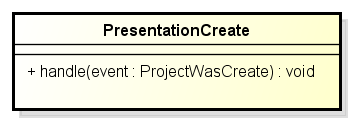
\includegraphics[width=0.5\linewidth]{img/premi_back_end_presentation_create}
	\caption[Diagramma della classe PresentationCreate]{Diagramma della classe PresentationCreate}
	\label{fig:premi_back_end_presentation_create}
\end{figure}


\paragraph{Descrizione}
La classe PresentationCreate risponde all'evento ProjectWasCreate e crea una presentazione associata al progetto appena creato.

\paragraph{Utilizzo}
Utilizzata quando viene creato un nuovo progetto e lanciato l'evento ProjectWasCreated.

\paragraph{Metodi:}
\begin{itemize}
	\item \textbf{+ handle(event: ProjectWasCreated) : void}\\
	Crea una nuova presentazione associata al progetto contenuto, e che ha invocato, l'evento ProjectWasCreated:\\
	\textbf{Argomenti:}
	\begin{itemize}
		\item project : Project;
		L'evento che ha chiamato il listener.
	\end{itemize}
\end{itemize}

\newpage
\subsubsection{SlideCreate}
\begin{figure}[h]
	\centering
	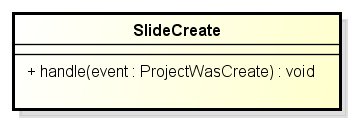
\includegraphics[width=0.5\linewidth]{img/premi_back_end_slide_create}
	\caption[Diagramma della classe SlideCreate]{Diagramma della classe SlideCreate}
	\label{fig:premi_back_end_slide_create}
\end{figure}


\paragraph{Descrizione}
La classe SlidCreate risponde all'evento ProjectWasCreate e crea una prima \gls{slide} di default all'interno della presentazione associata al progetto appena creato.

\paragraph{Utilizzo}
Utilizzata quando viene creato un nuovo progetto e lanciato l'evento ProjectWasCreated.

\paragraph{Metodi:}
\begin{itemize}
	\item \textbf{+ handle(event: ProjectWasCreated) : void}\\
	Crea una prima \gls{slide} di default della presentazione associata al progetto contenuto, e che ha invocato, l'evento ProjectWasCreated:\\
	\textbf{Argomenti:}
	\begin{itemize}
		\item project : Project;
		L'evento che ha chiamato il listener.
	\end{itemize}
\end{itemize}
